\documentclass{beamer}
%
% Choose how your presentation looks.
%
% For more themes, color themes and font themes, see:
% http://deic.uab.es/~iblanes/beamer_gallery/index_by_theme.html
%
\mode<presentation>
{
  \usetheme{default}      % or try Darmstadt, Madrid, Warsaw, ...
  \usecolortheme{default} % or try albatross, beaver, crane, ...
  \usefonttheme{default}  % or try serif, structurebold, ...
  \setbeamertemplate{navigation symbols}{}
  \setbeamertemplate{caption}[numbered]
} 

\usepackage{polski}
\usepackage{listings}
\lstset{language=Matlab}          % Set your language (you can change the language for each code-block optionally)

\usepackage{sansmathaccent}
\pdfmapfile{+sansmathaccent.map}

\usepackage[utf8x]{inputenc}

\title[SKORKA]{System wspomagający firmę sprzedającą i produkującą materiały powlekane}
\author{Rafał \textsc{Grabiański}, Zbigniew \textsc{Królikowski}, Paulina \textsc{Żak}}
\institute{}
\date{17.06.2015}

\begin{document}

\begin{frame}
  \titlepage
\end{frame}

% Uncomment these lines for an automatically generated outline.
%\begin{frame}{Outline}
%  \tableofcontents
%\end{frame}

\section{Obszar modelowania}

\begin{frame}{Struktura organizacyjna przedsiębiorstwa}

\begin{block}{Schemat organizacji}
\centering
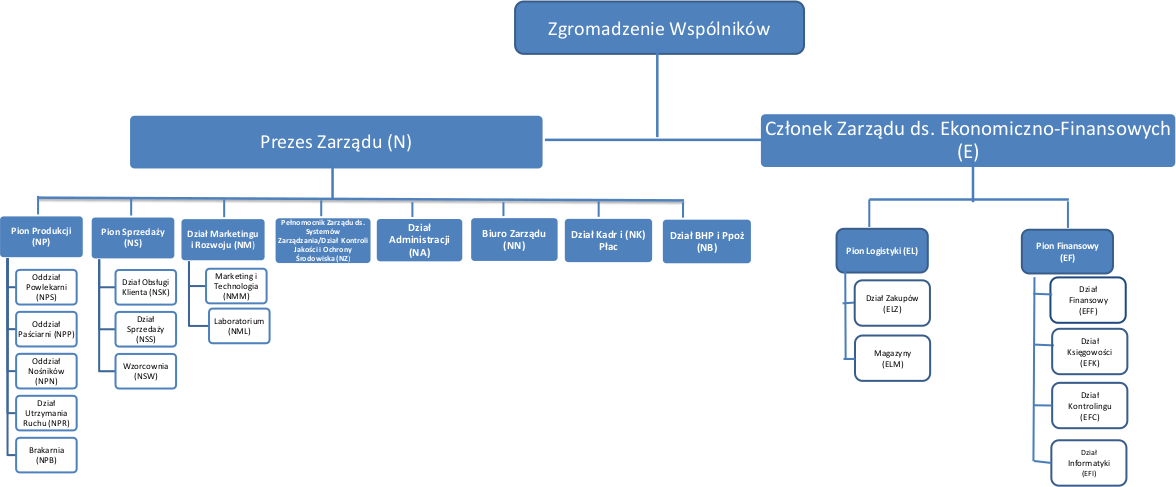
\includegraphics[scale=0.25]{schemat.png}
\end{block}

\end{frame}

\begin{frame}{Obszary aktywności}

\begin{itemize}
\item Wspmaganie sprzedaży
\item Wspomaganie produkcji
\item Wspomaganie zakupu surowców
\item Zarządzanie pracą
\item Wspomaganie pracy magazynów
\end{itemize}

\end{frame}

\begin{frame}{Analiza wymagań funkcjonalnych}
\begin{block}{Wspomaganie sprzedaży}
\centering
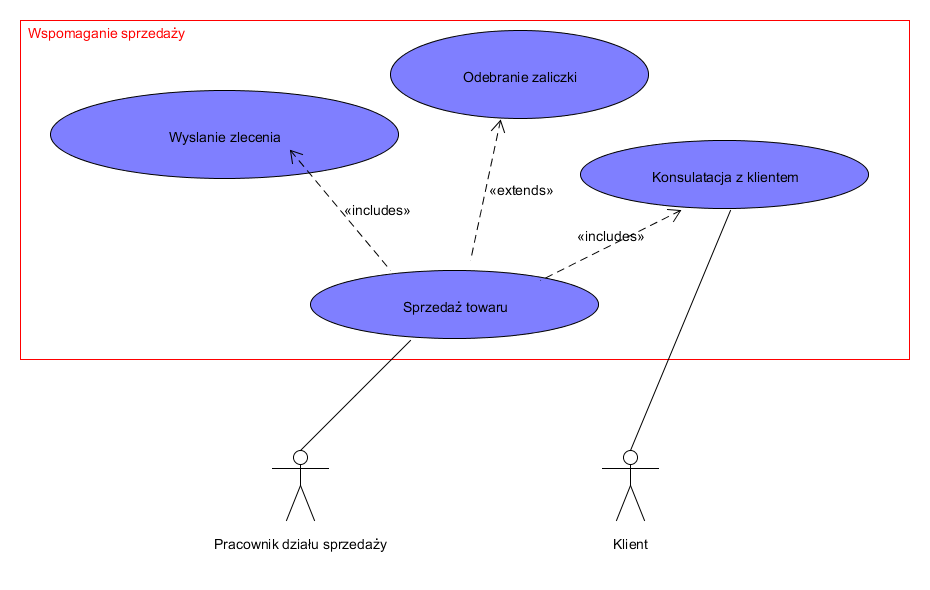
\includegraphics[scale=0.25]{Sprzedaz_towaru.png}
\end{block}


\end{frame}

\begin{frame}{Diagramy DFD}
\begin{block}
\centering
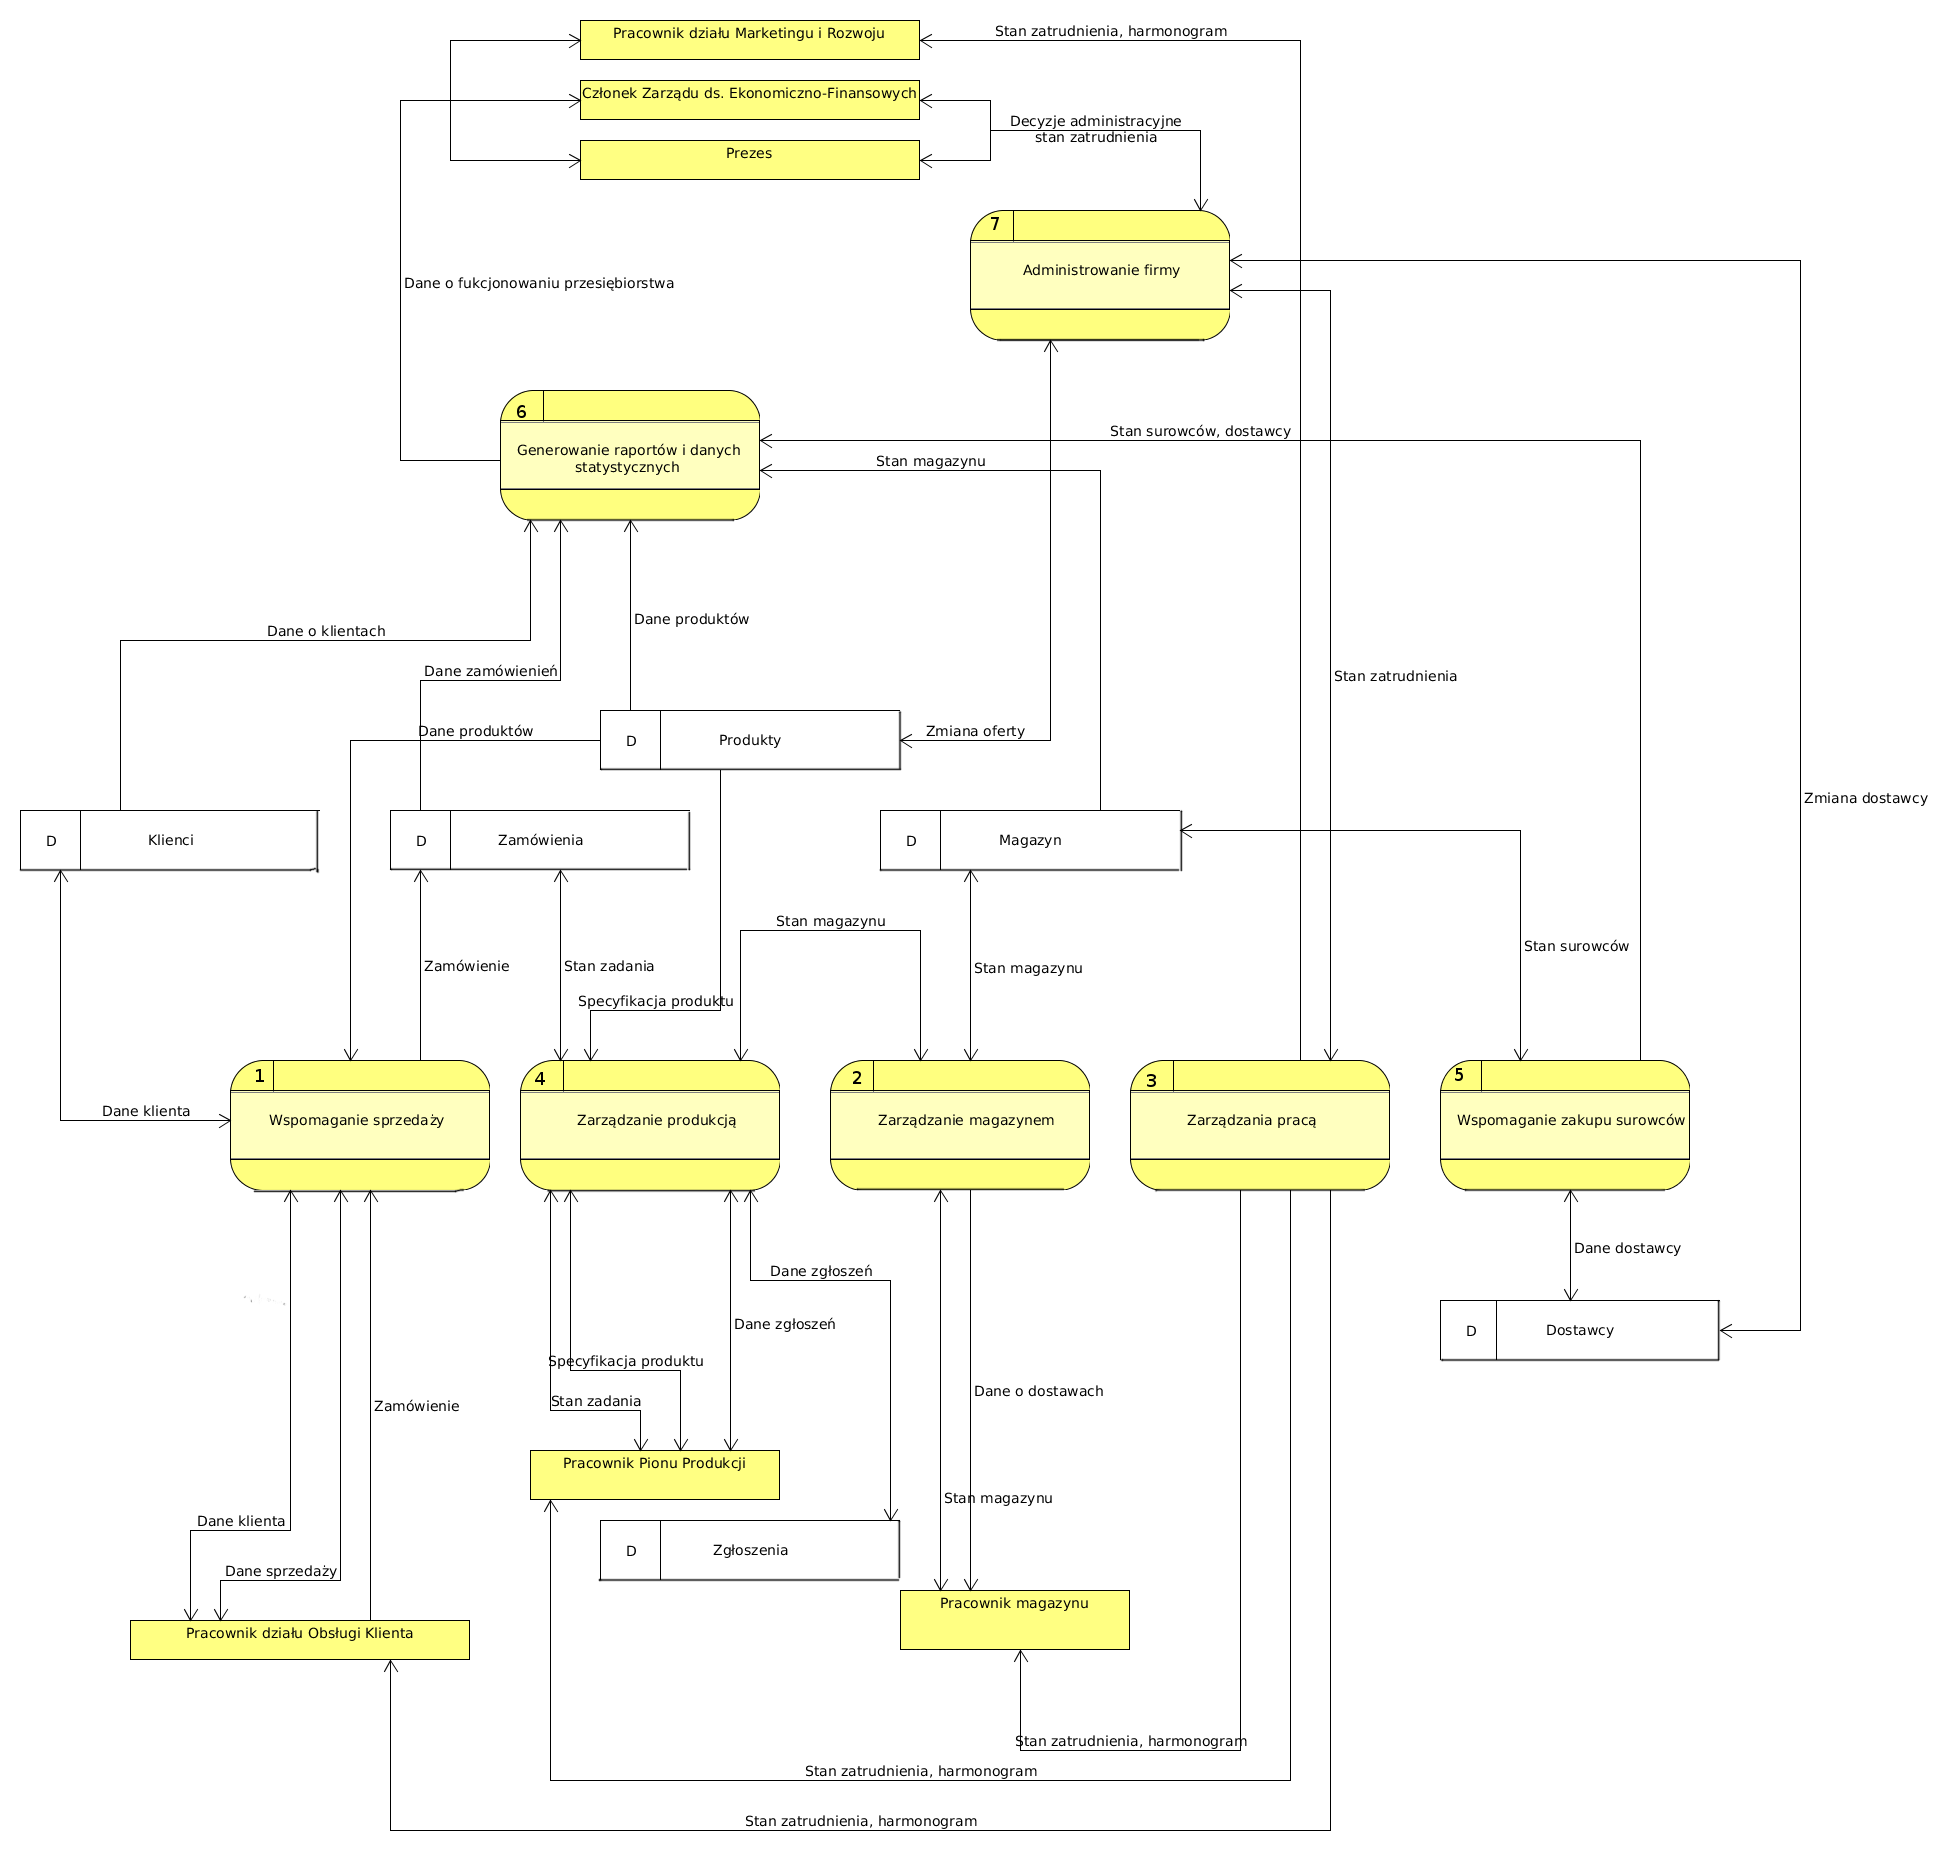
\includegraphics[scale=0.12]{DFD0.png}
\end{block}
\end{frame}


\begin{frame}{Analiza struktur danych przechowywanych w magazynach}
\begin{block}
\centering
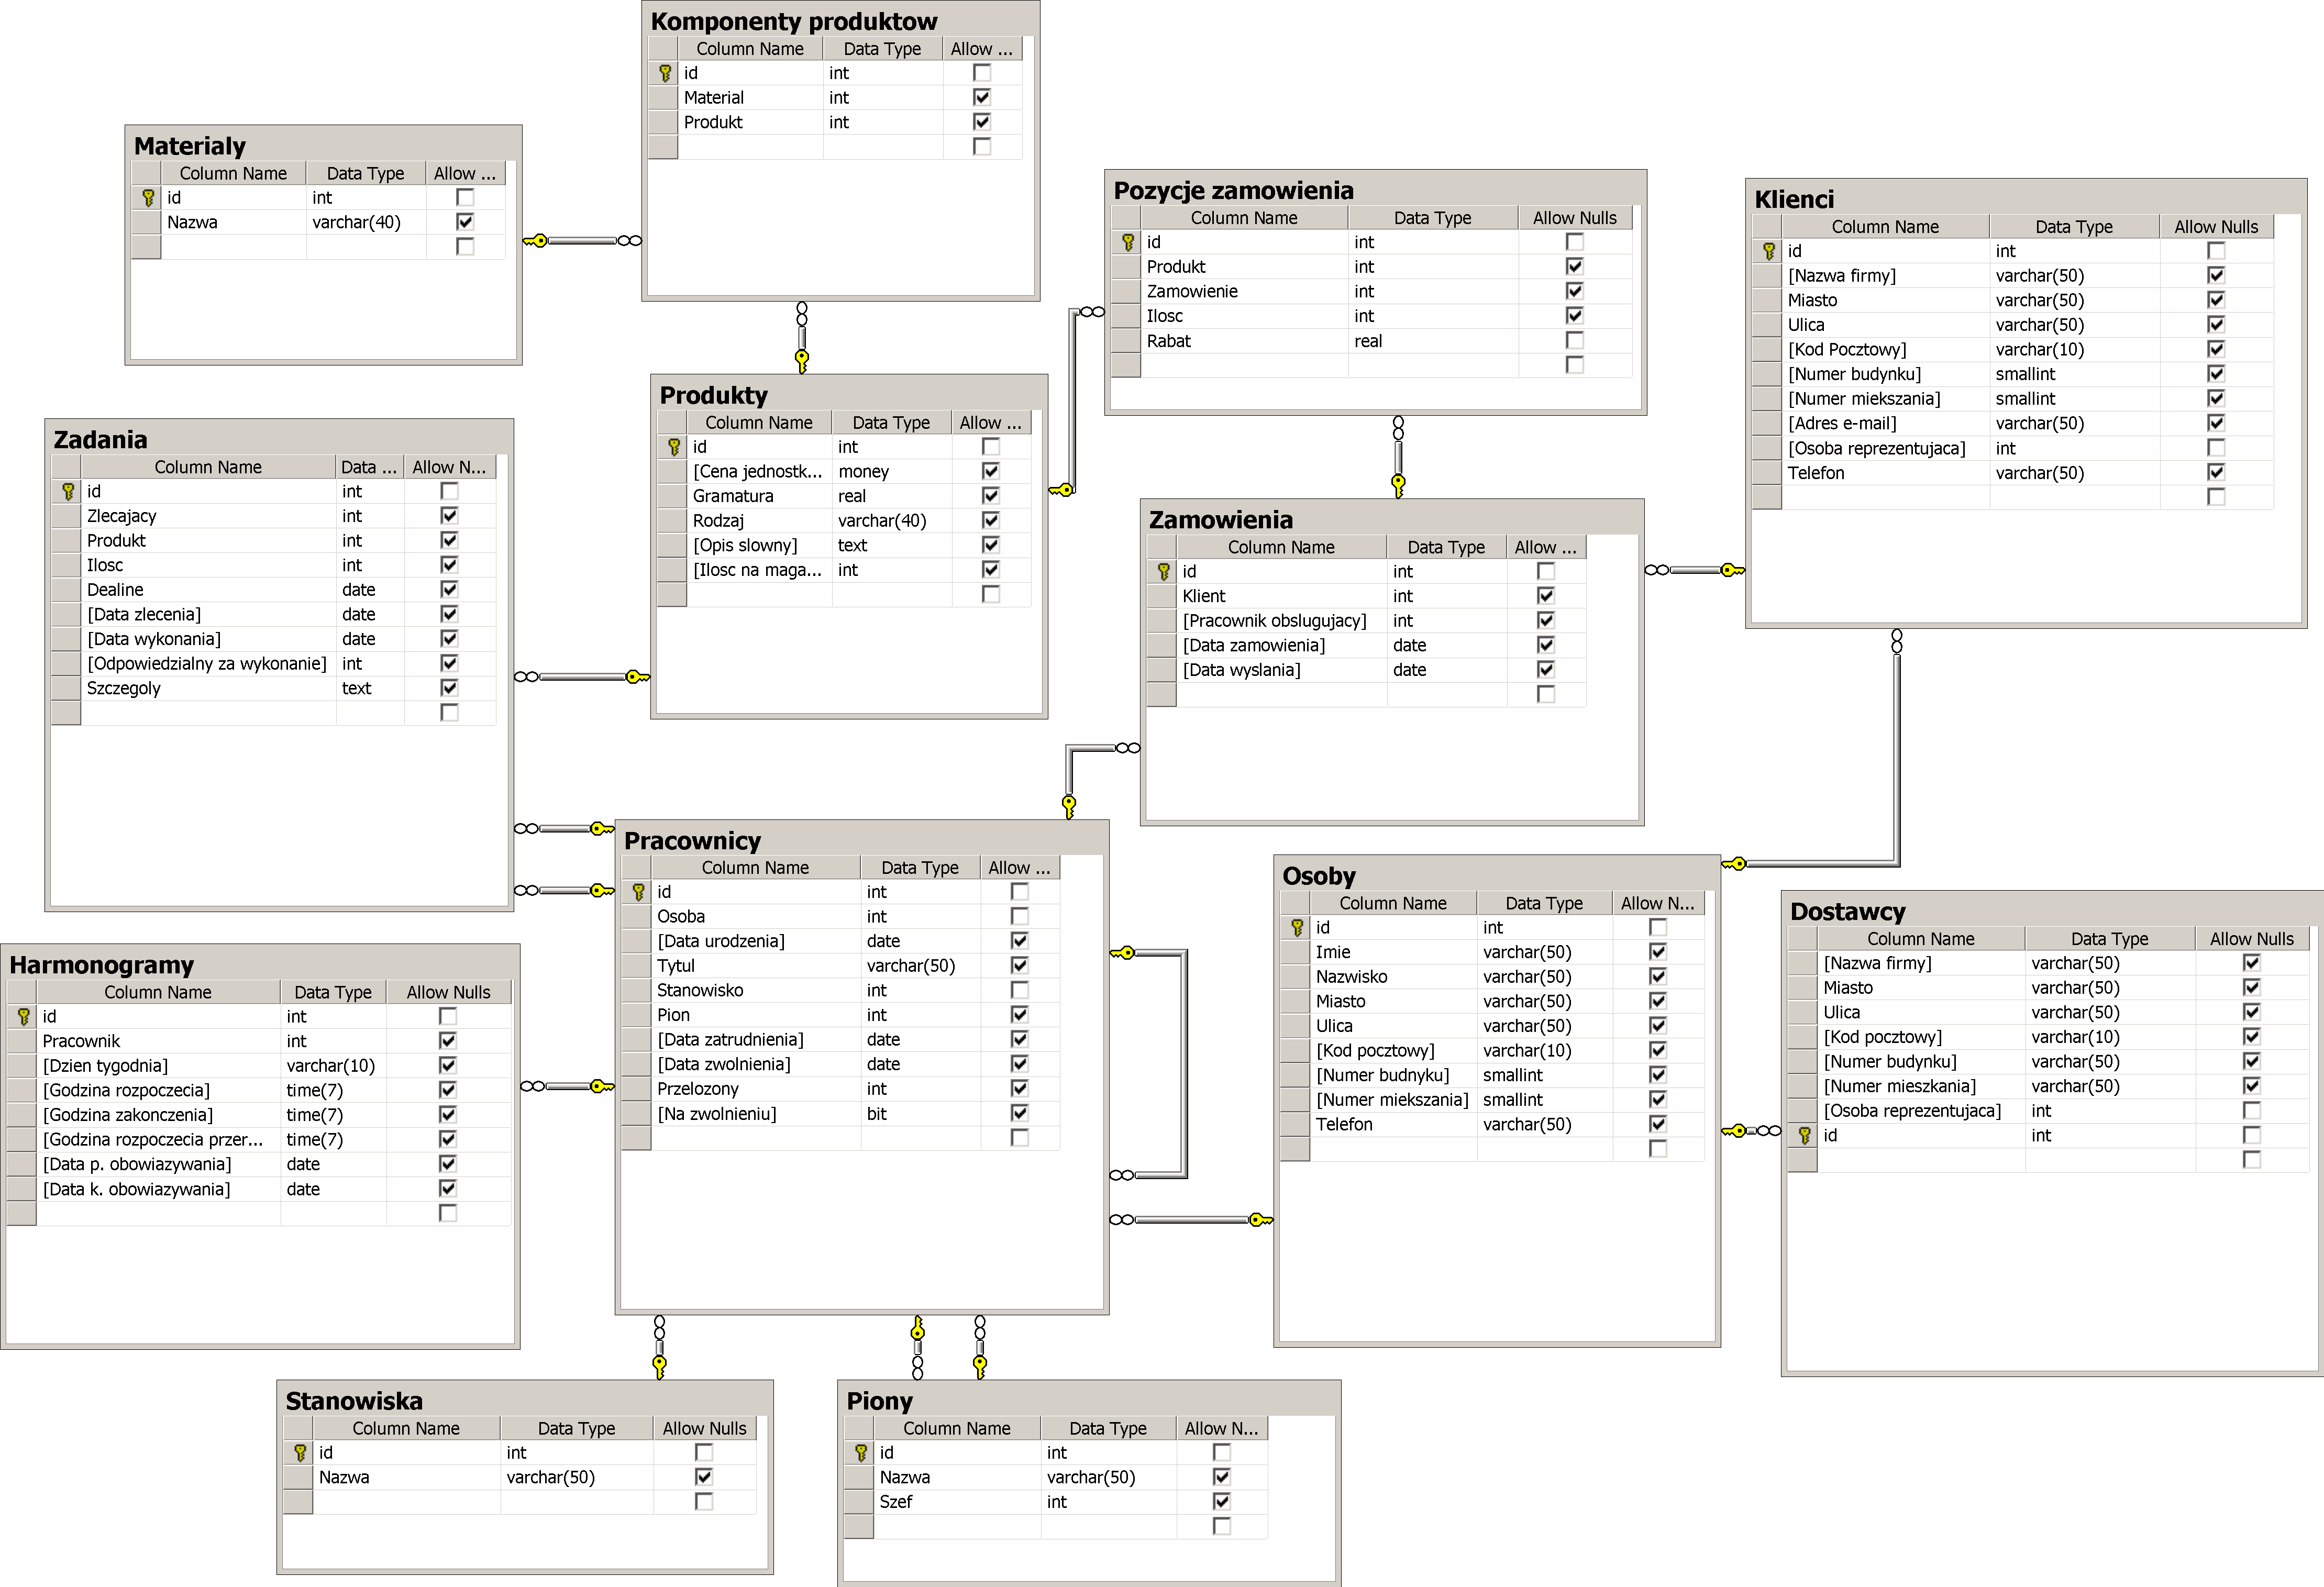
\includegraphics[scale=0.09]{diagram.png}
\end{block}
\end{frame}

\begin{frame}{Przykładowy Activity Diagram}
\begin{block}
\centering
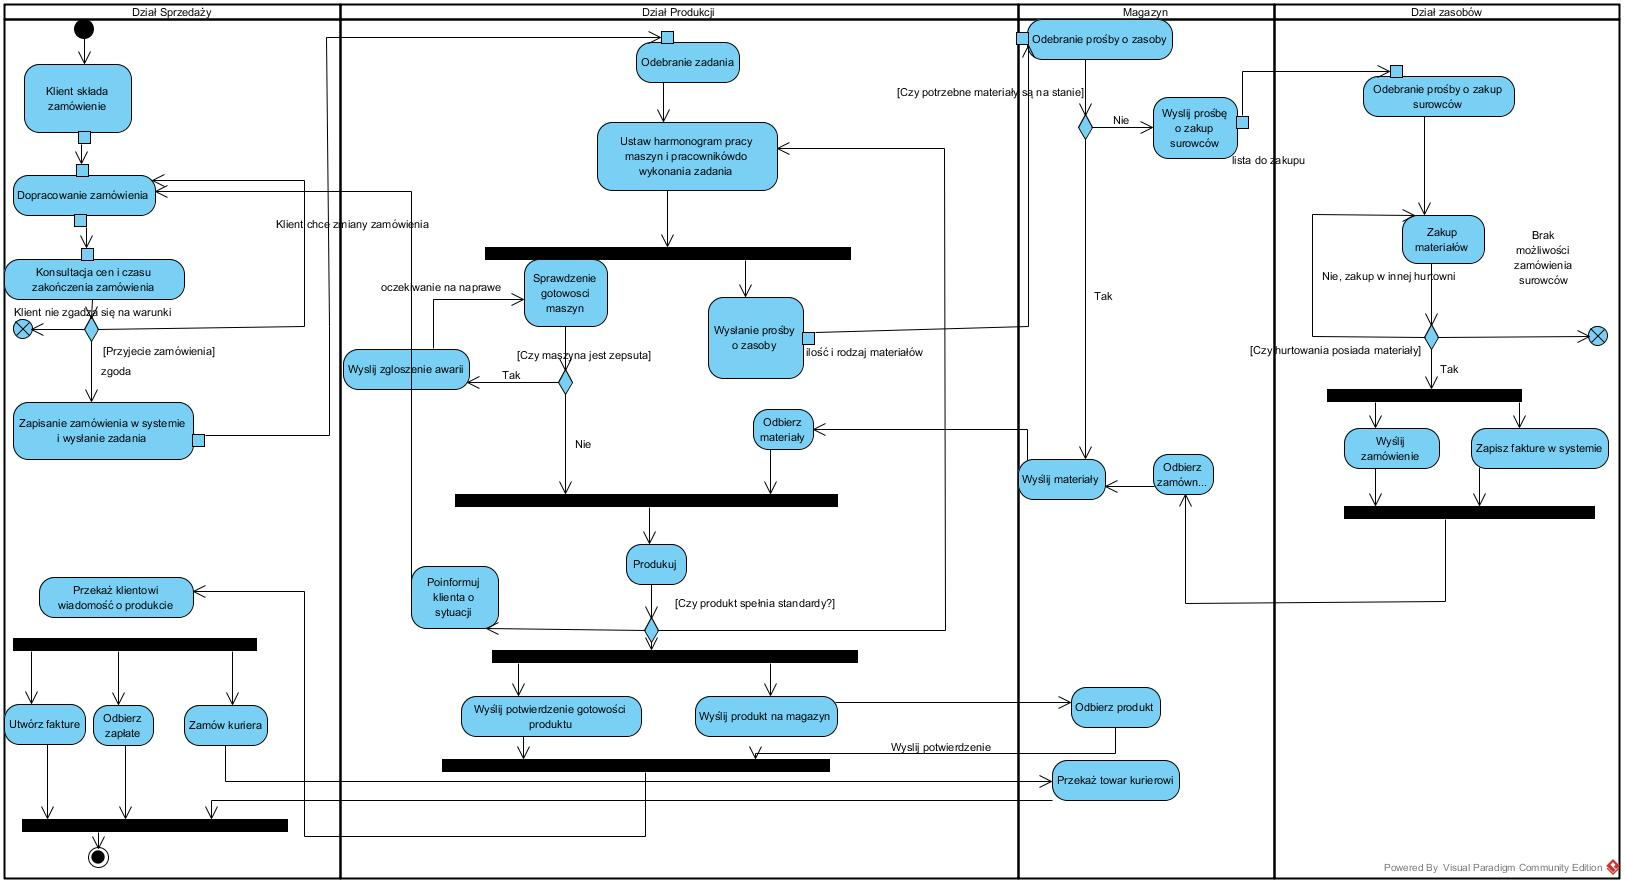
\includegraphics[scale=0.19]{Sprzedaz.jpg}
\end{block}
\end{frame}

\begin{frame}{GUI}
\begin{block}
\centering
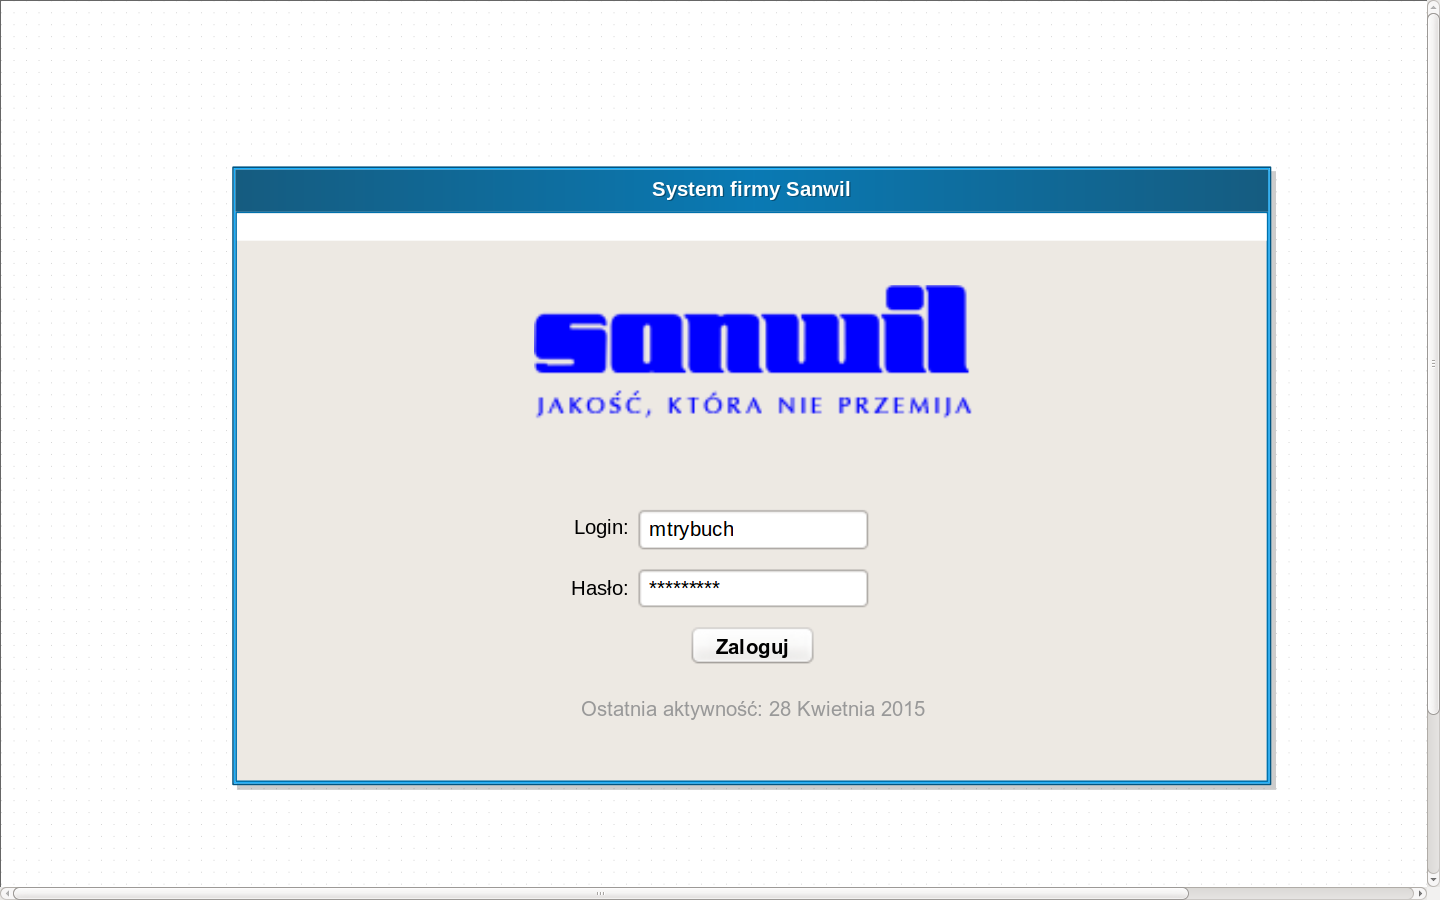
\includegraphics[scale=0.19]{logowanie.png}
\end{block}
\end{frame}

\begin{frame}{GUI}
\begin{block}
\centering
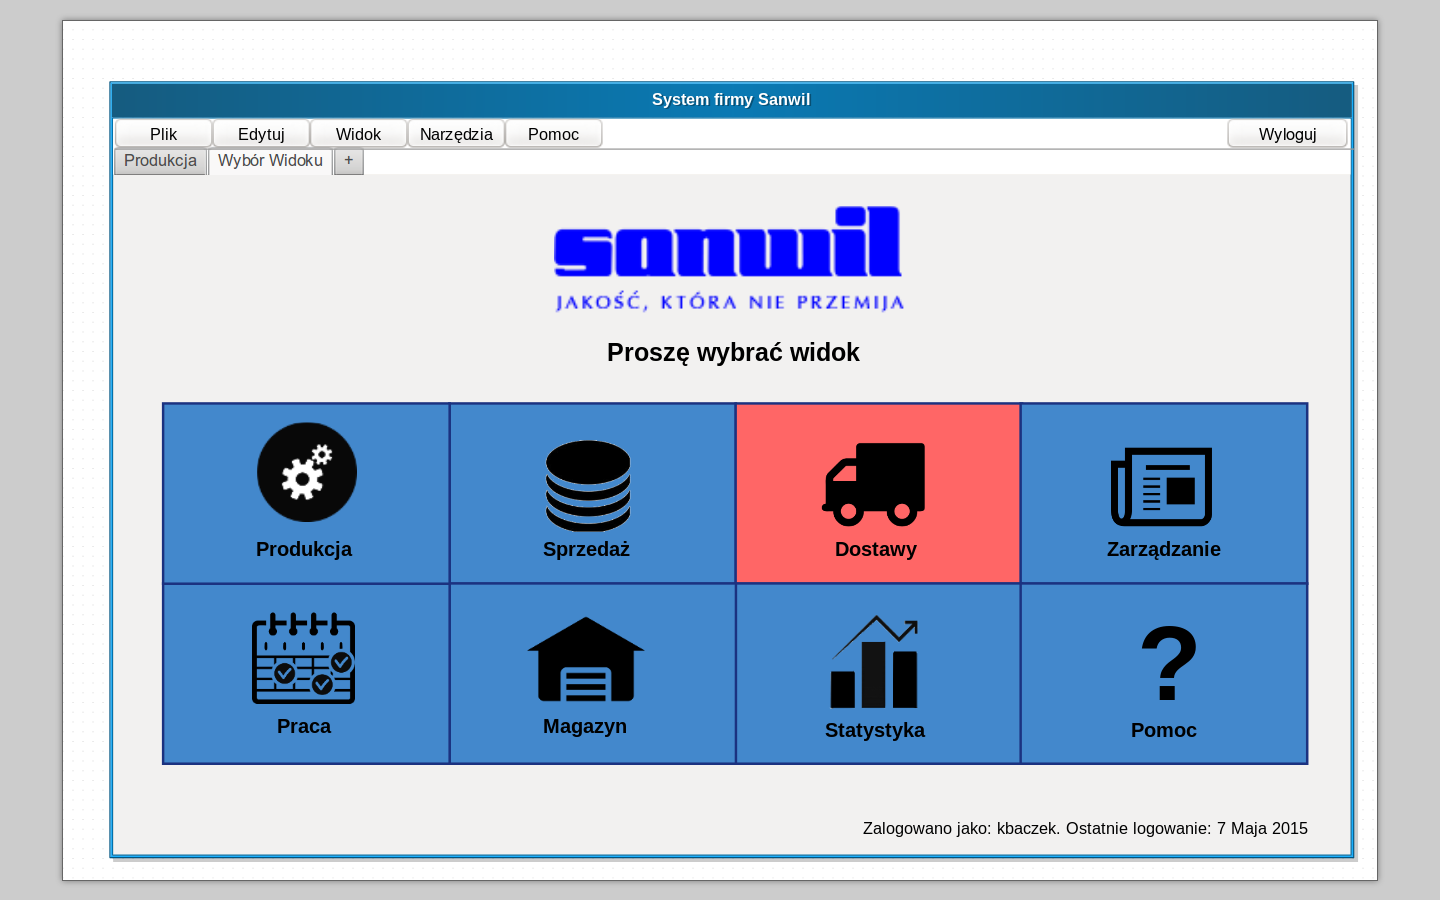
\includegraphics[scale=0.19]{nowa_karta.png}
\end{block}
\end{frame}

\begin{frame}{GUI}
\begin{block}
\centering
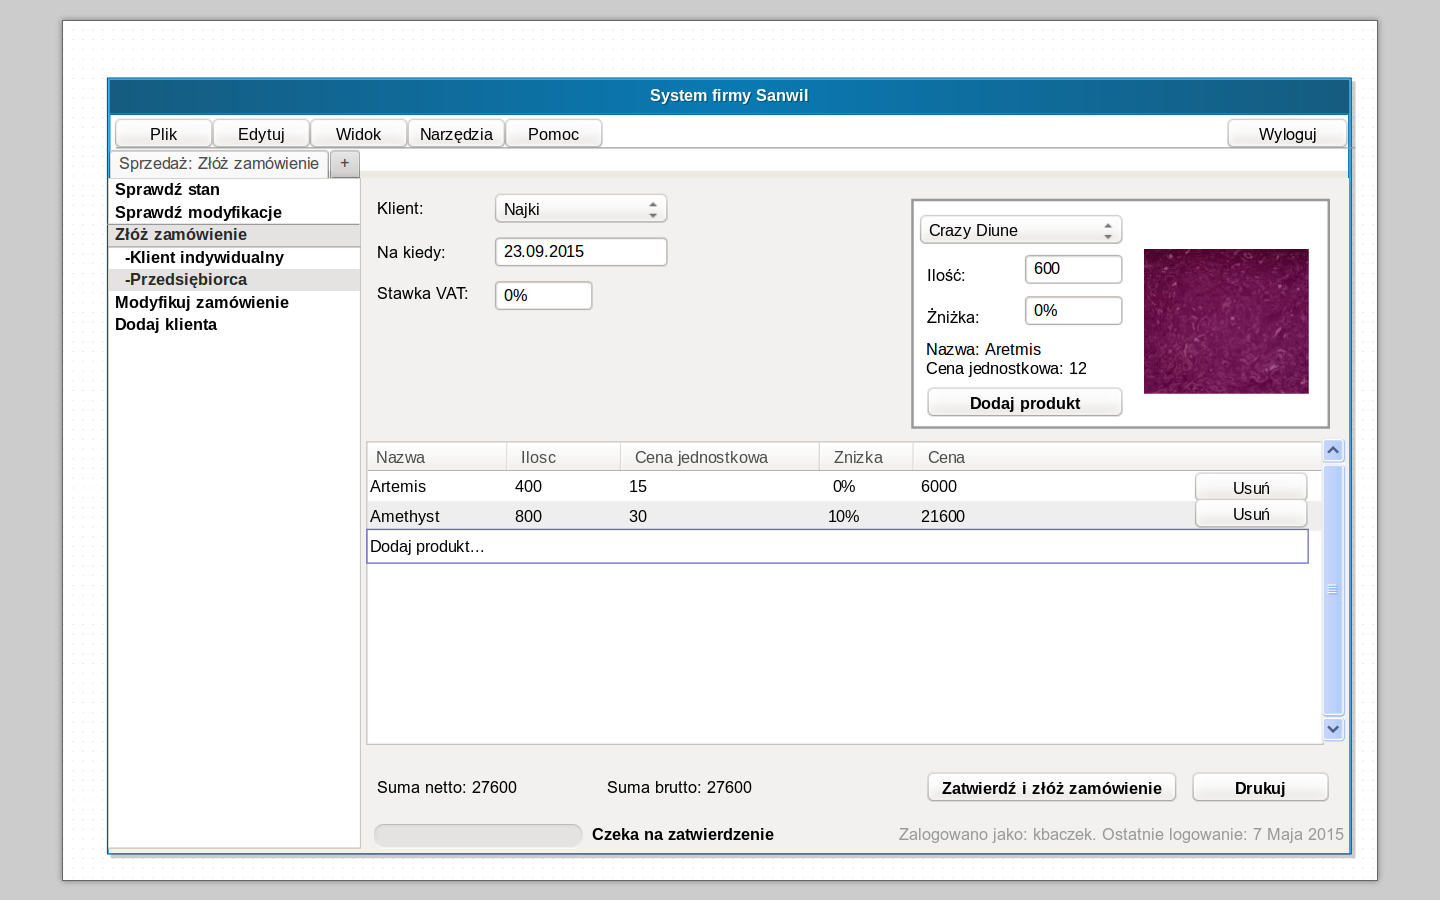
\includegraphics[scale=0.19]{sprzedaz.png}
\end{block}
\end{frame}

\begin{frame}{GUI}
\begin{block}
\centering
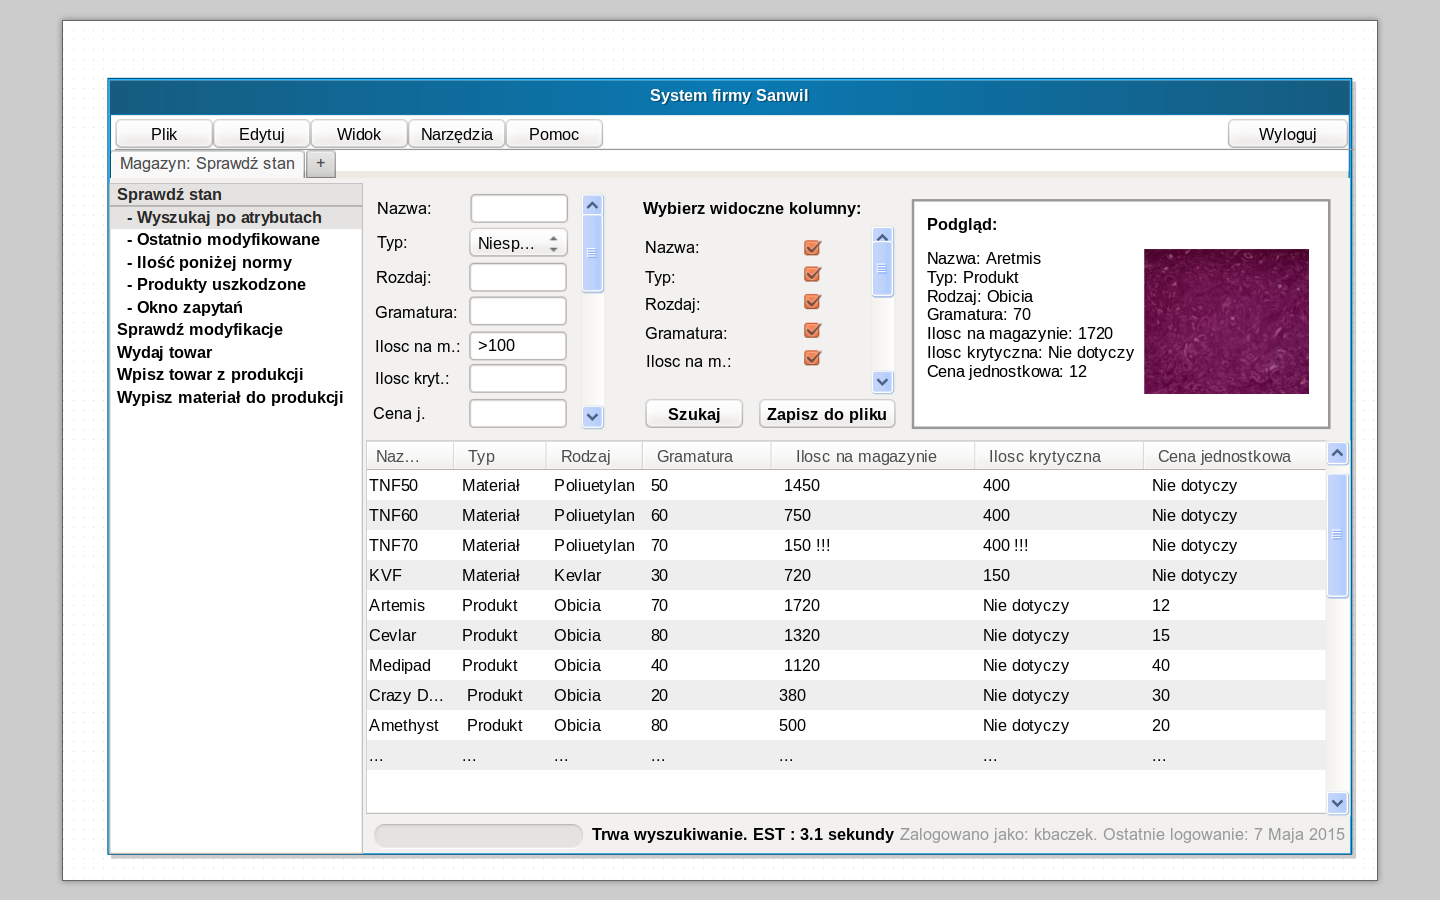
\includegraphics[scale=0.19]{magazyn.png}
\end{block}
\end{frame}


\end{document}
